\section{Introduction}
Bomberman is a game originally created and published by Hudson Soft inc. in the United Kingdom in the year 1983. At this first introduction the game was called "Eric and the Floaters". The game was re-released later as "Bomberman" . The game became a huge hit and was recreated numerous of times by several different companies including Hudson Soft inc. \cite{mobygames}.\\

The goal of the game is to 'kill' the opponent by hitting them with an exploding bomb. Different versions of the game made it more difficult to reach the opponent by using for example crates that block the player from walking. This increases the time before players can start attacking each other.\\

All team members of the A5 group played this game as a kid. This created a mutual interest to create this game using only hardware. This will be done by first creating the game in VHDL. After that the VHDL will be synthesized and tested on an FPGA. If everything is working properly, the game will be created on a wafer which uses 180nm technology. \\%is this true??

In this report, a brief outline of the design process will be discussed.\\

%\begin{figure}[h]
 %   \centering
  %  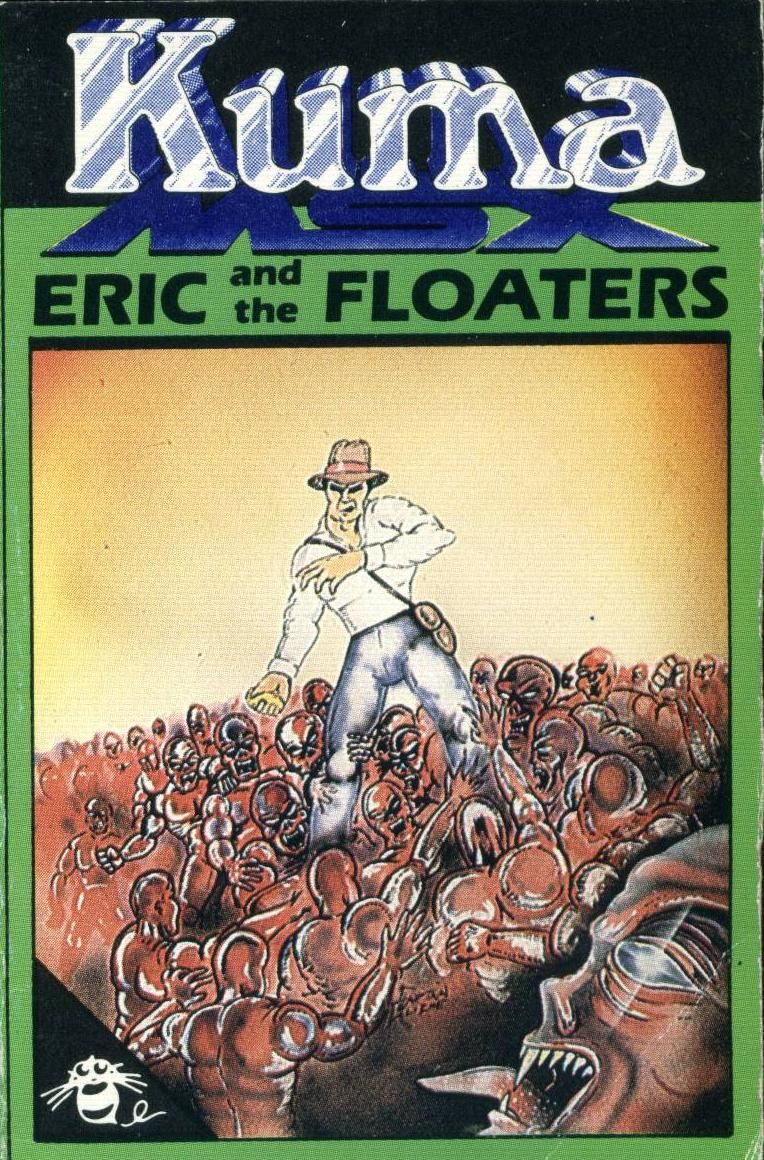
\includegraphics[width=40mm]{Figures/ericfloaters.jpg}
   % \caption{The front cover of the first bomberman game}
    %\label{fig:first}
%\end{figure}


\section{Global overview: Specification \& boundaries of the system}
\begin{figure}[H]
\begin{subfigure}{.5\textwidth}
    \centering
    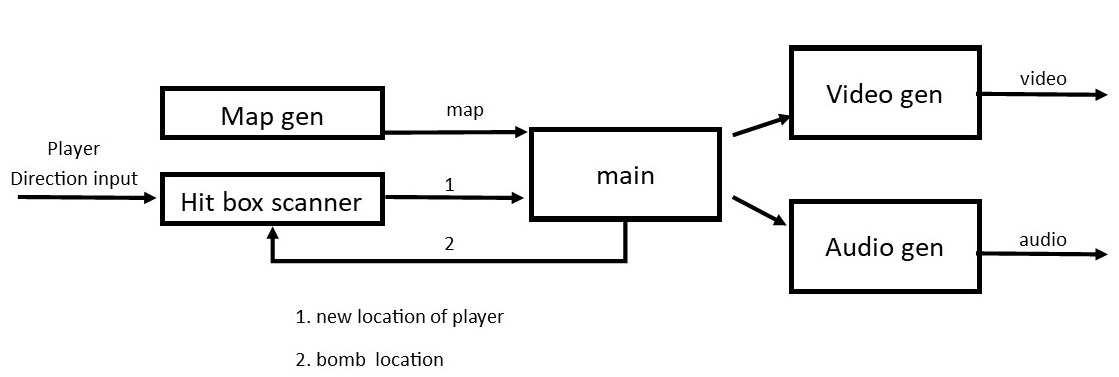
\includegraphics[width=1\linewidth]{Figures/function_block_diagram.jpg}
    \caption{The functional block diagram of the sub-blocks of the bomberman game with inputs, outputs and internal signals defined by arrows.}
    \label{fig:blockdiagram}
    \end{subfigure}% 
    \begin{subfigure}{.5\textwidth}
    \centering
    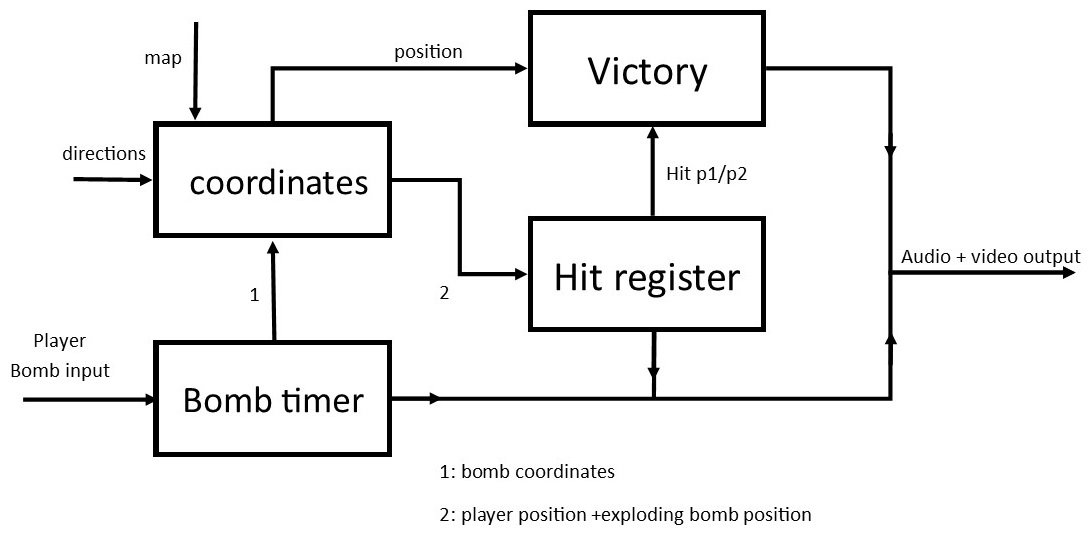
\includegraphics[width=1\linewidth]{Figures/main_block.jpg}
    \caption{The expanded functional block diagram of the main module from Fig. \ref{fig:blockdiagram} with input and outputs defined by arrows.}
    \label{fig:mainblockdiagram}
\end{subfigure}
\end{figure}

The goal is to create a 2-player multiplayer bomberman game. Each player has to be able to move in 4 directions and place bombs. For this, 5 inputs are needed per player. Adding the clock and reset input, a total of 12 inputs is needed. With 16 inputs available, this is not a problem. The reset input will put all Finite State Machines (in short: FSM's) in the reset state and can be used when a game is finished to restart the game. To visually interface with the user, an image is projected on a display through VGA. Optionally sound effects and a victory screen can be added. VGA requires 5 pins to work properly, this is not a problem with the total of 16 output pins. The audio should also be perfectly possible to implement with the amount of output pins that are available.\\

The maximum clock frequency of the chip is 12.5 MHz, which is not sufficient for the pixel-frequency of the VGA. This requires a clock frequency of 25 MHz. This will be resolved by reducing the resolution of the output. The resolution can be reduced, seen as the image quality of our game is not the focus of the project.\\

The FSM's must be a Moore machines. This means that the output of each FSM can only depend on the state of the machine, not on the input of the machine. The FSM's work at the rising clock edge, so all subsystems will be synchronized. \\

The size of the chip technology limits the amount of flipflops that can be used in the design. The maximum would be around 600 flipflops. This means that everything concerning signals and variables must be as efficient as possible in order to waste as few flipflops as possible. This is very crucial in a lot of modules, for example the coordinates of grid.

The general idea of the system is that the input of movement of the players should be checked by the \textbf{hitbox} module in Fig. \ref{fig:blockdiagram}. If it is possible to move, the \textbf{hitbox} passes the new coordinates to the \textbf{main} module. This module consists of the \textbf{coordinates}, \textbf{bomb timer}, \textbf{victory} and \textbf{Hit register} sub-modules, these are further explained in Section \ref{overview}. 